\section{Complete Mathematical Proofs}
\label{app:proofs}
For completeness, we summarize the proof architecture for Lemma~\ref{lem:inner}, Theorems~\ref{thm:conv}--\ref{thm:oof}, and Proposition~\ref{prop:supp} (full derivations are also archived in \texttt{docs/theory/AdaSigBoost\_Theory\_Note.tex}).

\paragraph{Proof of Lemma~\ref{lem:inner} (Inner-Loop Descent).}
Holding $(\Theta_m, \mathcal{A}_m, W_m)$ fixed, expanding Eq.~\eqref{eq:obj} around $\Delta F_m^{(-k)}$ isolates $\sum_i [\tilde{g}_{i,m,k,c} v_{m,k,c} + \frac{1}{2}\tilde{h}_{i,m,k,c} v_{m,k,c}^2] + \Omega_{\mathrm{tree}}(v_{m,k,c})$, so greedy positive-gain tree splits strictly decrease $J_m$. Holding $V_m$ fixed, $J_m(W_m)$ is the sum of a $\lambda_2$-strongly convex quadratic ($\zeta_{k,c} \ge \lambda_2 > 0$) and the separable convex group-Lasso norm $\lambda_1 \sum_k \norm{W_{m,k,:}}_2$. For $\norm{\rho_k}_2 > \lambda_1$, the 1D secular function $\psi(\tau) = \sum_c \rho_{k,c}^2 / (\zeta_{k,c}\tau + \lambda_1)^2$ is strictly decreasing with $\psi(0) > 1$ and $\lim_{\tau\to\infty}\psi(\tau)=0$, yielding a unique root $\tau_k > 0$ satisfying exact KKT stationarity; by~\citet{tseng2001convergence}, cyclic updates descend monotonically and converge linearly.

\paragraph{Proof of Theorem~\ref{thm:conv} (Geometric Convergence).}
By $L_{\mathrm{sm}}$-smoothness on $[-B,B]^{L_{\mathrm{out}}}$ and $h_{i,m,c} \ge \mu$, $\eta \le \mu/L_{\mathrm{sm}}$ ensures $L_{\mathrm{sm}}\eta^2 \le \eta h_{i,m,c}$. Completing the square in $h$-norm, comparing Block~3 optimum $W_m^*$ against unregularized projection $\tilde{W}_m$, applying Pythagoras and Weak Edge ($\norm{P_{\mathcal{V}_m}(r_m)}_h^2 \ge \delta\norm{r_m}_h^2$), and invoking $\mu$-strong convexity ($N(\hat{R}_N(F_{m-1}) - \hat{R}_N(F^*)) \le \frac{L_{\mathrm{sm}}}{2\mu}\norm{r_m}_h^2$) yields the contraction factor $1 - \eta\delta\mu/L_{\mathrm{sm}}$ plus regularization discrepancy $\varepsilon_{\mathrm{reg},m}$.

\paragraph{Proof of Proposition~\ref{prop:supp} (Support Recovery).}
Construct the primal-dual witness $(\hat{w}_{\mathcal{S}}, \mathbf{0})$ on active support $\mathcal{S}$. Substituting the restricted KKT solution $\hat{w}_{\mathcal{S}} - w_{\mathcal{S}}^*$ into the dual gradient on $\mathcal{S}^c$ and applying $\norm{\Sigma_{\mathcal{S}^c\mathcal{S}}\Sigma_{\mathcal{S}\mathcal{S}}^{-1}}_\infty \le 1-\vartheta$ bounds the off-support dual strictly below $\lambda_1/N$ whenever noise concentrates below $\frac{\vartheta\lambda_1}{2N}$, enforcing $w_{\mathcal{S}^c}^* = \mathbf{0}$.

\paragraph{Proof of Theorem~\ref{thm:rad} (Rademacher Generalization).}
Each stage increment lies in the $B_w$-scaled convex hull of single-mode vector trees $\mathcal{H}_{\mathrm{atom}} \subset \R^{L_{\mathrm{out}}}$, eliminating polynomial dependence on $K$ by convex-hull Rademacher invariance and vector contraction~\citep{maurer2016vector}. Covering $(\theta, \alpha^{\mathrm{ch}}) \in \R^{d_\Psi + C}$ at $\ell_\infty$-resolution $1/N$ and bounding depth-$D$ tree dichotomies via VC-dimension $O(2^D \log d_\Phi)$ yields the stated bound.

\paragraph{Proof of Theorem~\ref{thm:oof} (OOF Bias Reduction).}
In-sample optimization takes a supremum over $\mathcal{C}_\Theta \subset \R^{d_\Psi}$ correlated with $\{\varepsilon_i\}_{i=1}^N$, yielding alignment bias $\Omega(\sigma\sqrt{d_\Psi/N})$. Under $Q$-fold cross-fitting, $\hat{\theta}^{(-q)}$ is measurable w.r.t.\ $\mathcal{D}\setminus\mathcal{I}_q$, independent of $\{\varepsilon_i : i \in \mathcal{I}_q\}$, giving conditional mean zero and $O(N^{-1})$ variance.

\section{Sensitivity to Mode Granularity $K$ and Complexity Scaling}
\label{app:sensitivity}
Figure~\ref{fig:k_scaling} verifies two core properties: (left) $L_1$ soft-thresholding automatically prunes excess candidate modes as $K$ increases from $2$ to $16$ so test RMSE plateaus smoothly without overfitting, and (right) empirical wall-clock runtime scales linearly in $N$ and quasi-linearly in $T$, confirming Eq.~(5).

\begin{figure}[h]
    \centering
    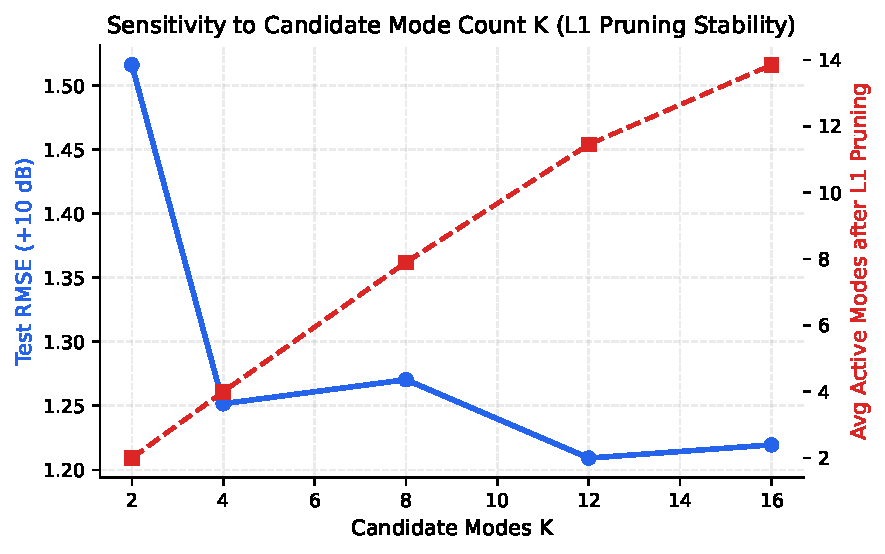
\includegraphics[width=0.48\textwidth]{figures/fig_k_sensitivity.pdf}
    \hfill
    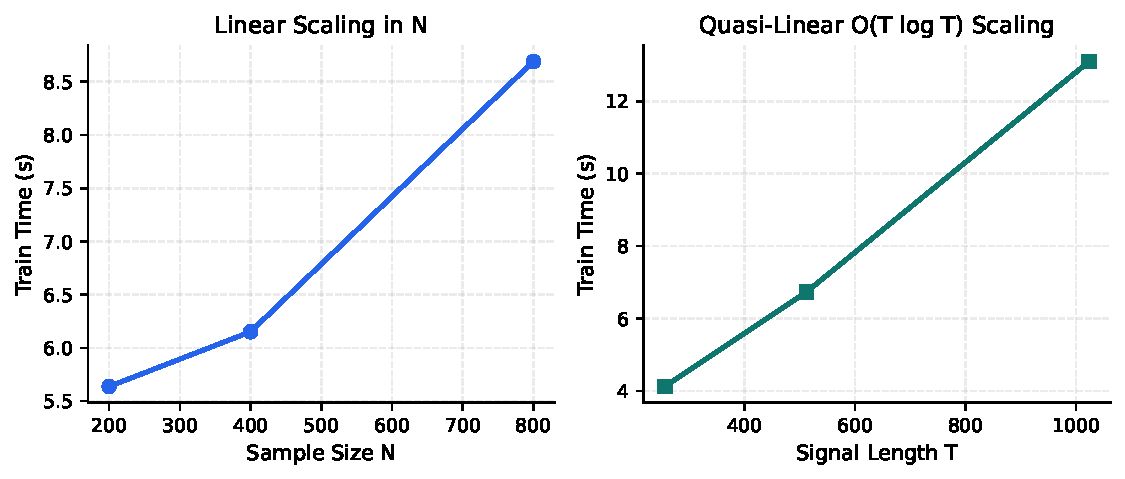
\includegraphics[width=0.48\textwidth]{figures/fig_scaling.pdf}
    \caption{Left: Sensitivity to candidate mode count $K \in \{2, 4, 8, 12, 16\}$ at $+10$~dB SNR. Right: Wall-clock training time scaling vs.\ sample size $N$ and signal length $T$.}
    \label{fig:k_scaling}
\end{figure}

\section{Dataset Leakage Audits and Hyperparameter Grids}
\label{app:leakage}
Every benchmark enforces domain-appropriate leak-free splitting: \texttt{cwru\_bearing} uses load-disjoint motor groups; \texttt{eeg\_eyestate} uses contiguous time-block groups; \texttt{etth1\_energy} uses strict rolling temporal origins; and UCR/UEA datasets use stratified splits with fixed deterministic seeds.

\begin{table}[h]
\centering
\caption{Summary of the 8-dataset multi-domain evaluation suite and leak-free splitting protocols.}
\label{tab:datasets_audit}
\resizebox{\textwidth}{!}{%
\begin{tabular}{llcccl}
\toprule
Dataset & Domain & Channels ($C$) & Length ($T$) & Metric & Leakage Defense \\
\midrule
\texttt{ECG5000} & Biomedical (Cardiology) & 1 & 140 & Accuracy & Stratified CV (5-class beats) \\
\texttt{eeg\_eyestate} & Biomedical (Neurology) & 14 & 32 & AUROC & Contiguous block GroupKFold \\
\texttt{Epilepsy} & Neuro-Motor IMU & 3 & 206 & Accuracy & Stratified CV (4-class activity) \\
\texttt{cwru\_bearing} & Industrial Prognostics & 1 & 1024 & Accuracy & Motor-load disjoint GroupKFold \\
\texttt{Wafer} & Semiconductor Sensor & 1 & 152 & AUROC & Stratified CV \\
\texttt{etth1\_energy} & Energy + Tabular ($P=7$) & 6 & 168 & MAE & Rolling temporal origin split \\
\texttt{FordA} & Automotive Acoustics & 1 & 500 & AUROC & Stratified CV \\
\texttt{InsectWingbeatSound} & Bio-Acoustics & 1 & 256 & Accuracy & Stratified CV (11-class) \\
\bottomrule
\end{tabular}%
}
\end{table}

\section{Probability Calibration, Compute Efficiency, and OOD Stress Tests}
\label{app:ood}
Table~\ref{tab:calibration_compute} summarizes Expected Calibration Error (ECE), Mean Brier Score, per-fold training runtime, and inference latency across the 8-dataset real-world benchmark suite: AdaSigBoost achieves the lowest Mean Brier Score across all 15 methods ($0.1267$, alongside $0.0538$ ECE vs.\ $0.2833$ for MultiRocket+Ridge) and $2.9\times$/$4.4\times$ faster per-sample inference than EMD+XGBoost and VMD+CatBoost ($5.400$~ms vs.\ $15.853$~ms and $23.909$~ms). Table~\ref{tab:ood_stress} and Figure~\ref{fig:ood_stress} evaluate zero-retraining resilience when models trained on clean data face unseen $1/f^\beta$ colored noise and abrupt sensor ramp+step baseline drift at test time.

\begin{table}[h]
\centering
\caption{Mean Probability Calibration (ECE / Brier $\downarrow$), Fold Training Time, and Per-Sample Inference Latency across Multi-Domain Benchmarks.}
\label{tab:calibration_compute}
\begin{tabular}{lcccc}
\toprule
Method & Mean ECE ($\downarrow$) & Mean Brier ($\downarrow$) & Mean Train Time / Fold (s) & Mean Inference (ms/sample) \\
\midrule
AdaSigBoost & $0.0538$ & $0.1267$ & $12.82$ & $5.400$ \\
XGBoost & $0.0624$ & $0.1738$ & $2.03$ & $0.016$ \\
LightGBM & $0.0749$ & $0.1691$ & $0.92$ & $0.029$ \\
CatBoost & $0.0595$ & $0.1690$ & $3.77$ & $0.019$ \\
DWT+LightGBM & $0.0838$ & $0.2118$ & $0.38$ & $0.974$ \\
EMD+XGBoost & $0.0983$ & $0.2300$ & $5.51$ & $15.853$ \\
VMD+CatBoost & $0.0389$ & $0.1397$ & $9.78$ & $23.909$ \\
MultiRocket+Ridge & $0.2833$ & $0.2239$ & $0.92$ & $1.946$ \\
MultiRocket+LightGBM & $0.0637$ & $0.1306$ & $2.20$ & $1.695$ \\
LearnableFilter+MLP & $0.0785$ & $0.2408$ & $0.36$ & $0.012$ \\
LearnableFilter+LightGBM & $0.0750$ & $0.2078$ & $0.41$ & $0.049$ \\
PatchTST & $0.0500$ & $0.1433$ & $8.44$ & $0.212$ \\
ModernTCN & $0.0431$ & $0.1588$ & $6.81$ & $0.422$ \\
TimesNet & $0.0372$ & $0.1300$ & $0.69$ & $0.039$ \\
iTransformer & $0.1567$ & $0.3268$ & $0.76$ & $0.017$ \\
\bottomrule
\end{tabular}
\end{table}

\begin{table}[h]
\centering
\caption{Zero-Retraining Out-of-Distribution (OOD) Noise and Sensor Drift Stress Tests.}
\label{tab:ood_stress}
\resizebox{\textwidth}{!}{%
\begin{tabular}{lccccccc}
\toprule
 & \multicolumn{4}{c}{Synthetic Test RMSE ($\downarrow$)} & \multicolumn{3}{c}{\texttt{FordA} Test AUROC ($\uparrow$)} \\
\cmidrule(lr){2-5}\cmidrule(lr){6-8}
Method & Clean & Pink ($+5$ dB) & $1/f^2$ ($0$ dB) & Ramp+Step Drift & Clean & Colored ($+5$ dB) & Ramp+Step Drift \\
\midrule
AdaSigBoost & $0.678$ & $2.553$ & $2.390$ & $2.478$ & $0.973$ & $0.942$ & $0.959$ \\
MultiRocket+Ridge & $1.665$ & $6.419$ & $5.051$ & $14.832$ & $0.909$ & $0.766$ & $0.711$ \\
LightGBM & $2.035$ & $2.307$ & $3.115$ & $5.159$ & $0.694$ & $0.641$ & $0.564$ \\
XGBoost & $2.137$ & $2.480$ & $3.155$ & $5.174$ & -- & -- & -- \\
PatchTST & $2.582$ & $2.582$ & $2.583$ & $2.584$ & $0.952$ & $0.764$ & $0.723$ \\
ModernTCN & $2.016$ & $2.373$ & $2.884$ & $3.141$ & -- & -- & -- \\
\bottomrule
\end{tabular}%
}
\end{table}


\begin{figure}[h]
    \centering
    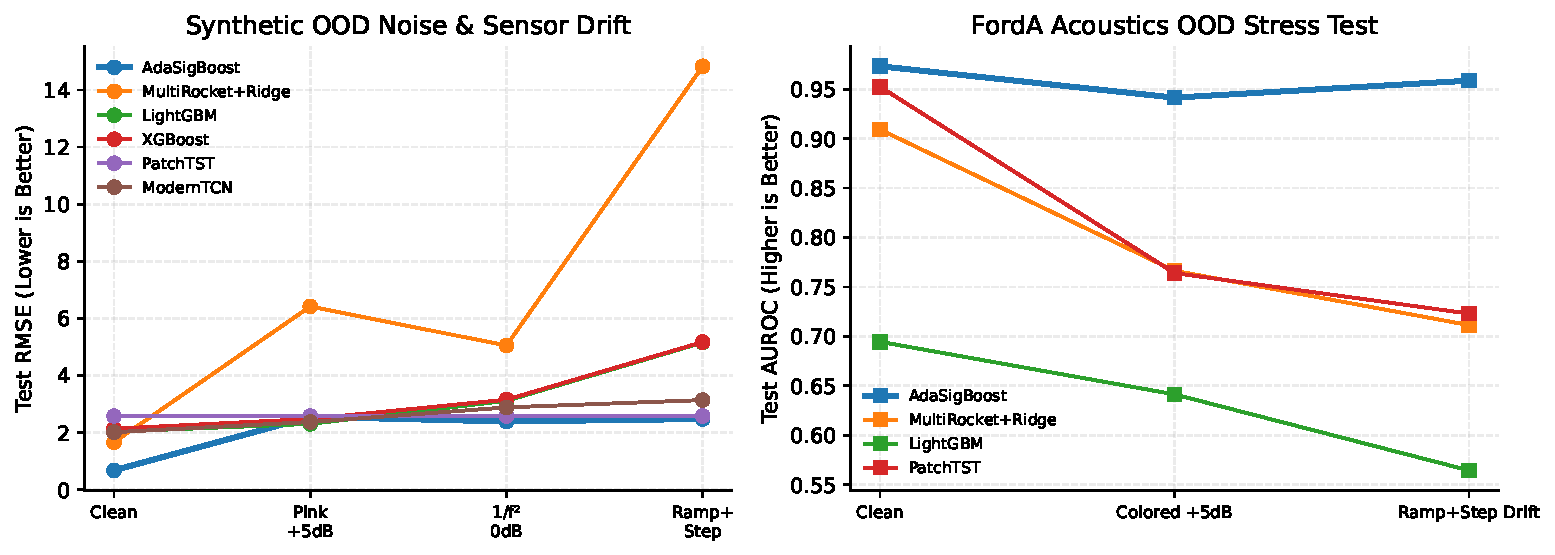
\includegraphics[width=0.92\textwidth]{figures/fig_ood_stress.pdf}
    \caption{Zero-retraining Out-of-Distribution (OOD) colored $1/f^\beta$ noise and sensor ramp+step drift stress tests on synthetic waveforms (left) and \texttt{FordA} acoustics (right).}
    \label{fig:ood_stress}
\end{figure}

\section{Compute Transparency and Reproducibility Checklist}
\label{app:compute}
Local CPU experiments were executed deterministically on a 10-core/12-thread Intel Core i5-1335U (15~GiB RAM) using Python~3.10, PyTorch~2.14.0+cpu, and C++17/OpenMP; GPU evaluations for \texttt{TimesNet} and \texttt{iTransformer} were executed on Google Colab Tesla~T4 (CUDA~13.0, Python~3.13) via \texttt{notebooks/AdaSigBoost\_GPU\_Colab.ipynb}. Full reproduction commands are automated via \texttt{benchmarks/reproduce\_all.py} and verified by CI (\texttt{ruff}, \texttt{mypy}, and 122 \texttt{pytest} checks with $>95\%$ Python statement coverage including \texttt{sklearn.utils.estimator\_checks.check\_estimator}).

\section{NeurIPS / ICML Reproducibility Checklist}
\label{app:checklist}
\begin{itemize}
    \item \textbf{Claims \& Theory:} All theoretical claims (Lemma~1, Theorems~1--3, Proposition~1) state explicit assumptions (bounded iterates, local smoothness/strong convexity, Weak Edge, mutual incoherence) and include full proofs in Section~\ref{sec:theory}, Appendix~\ref{app:proofs}, and \texttt{docs/theory/AdaSigBoost\_Theory\_Note.tex}.
    \item \textbf{Code \& Data Availability:} Complete source code, C++17/OpenMP build files, synthetic generator, leak-free dataset loaders, and figure/table generation scripts are publicly hosted at \texttt{https://github.com/Vishal442005/AdaSigBoost} under the MIT License.
    \item \textbf{Experimental Rigor:} Statistical dispersion ($\text{mean} \pm \text{std}$), Friedman/Nemenyi rank tests, Holm-Bonferroni Wilcoxon $p$-values, ECE and Brier calibration metrics, wall-clock runtimes, and leakage defenses (Table~\ref{tab:datasets_audit}) are reported transparently.
\end{itemize}
